% threepennygui-Ht.tex
\begin{hcarentry}[updated]{threepenny-gui}
\label{threepenny-gui}
\report{Heinrich Apfelmus}%11/14
\status{active development}
\makeheader

Threepenny-gui is a framework for writing graphical user interfaces (GUI) that uses the web browser as a display. Features include:

\begin{itemize}
\item \emph{Easy installation.} Everyone has a reasonably modern web browser installed. Just install the library from Hackage and you are ready to go. The library is cross-platform.
\item \emph{HTML.} You have all capabilities of HTML at your disposal when creating user interfaces. This is a blessing, but it can also be a curse, so the library includes a few layout combinators to quickly create user interfaces without the need to deal with the mess that is CSS. A small foreign function interface (FFI) for JavaScript allows you to include JS client libraries.
\item \emph{Functional Reactive Programming (FRP)} promises to eliminate the spaghetti code that you usually get when using the traditional imperative style for programming user interactions. Threepenny has an FRP library built-in, but its use is completely optional. Employ FRP when it is convenient and fall back to the traditional style when you hit an impasse.
\end{itemize}

\subsubsection*{Status}

The project is alive and kicking, the latest release is version \verb`0.5.0.0`. You can download the library from Hackage and use it right away to write that cheap GUI you need for your project. Here a screenshot from the example code:

%**<img width=700 src="./chat.jpg">
%*ignore
\begin{center}
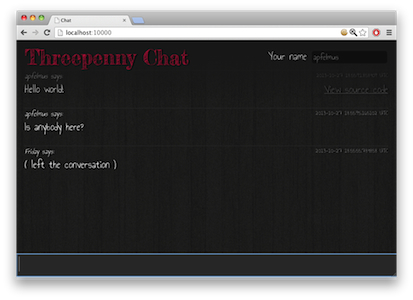
\includegraphics[width=0.5\textwidth]{html/chat.jpg}
\end{center}
%*endignore

For a collection of real world applications that use the library, have a look at the gallery on the homepage.

Compared to the previous report, the library now uses a \verb`UI` monad instead of the \verb`IO` monad. This simplifies many function signatures, in particular in the JavaScript FFI, and allows recursive uses of FRP. Moreover, the library now includes the full set of SVG elements and the beginnings of a small Canvas API.

\subsubsection*{Current development}

The library is still very much in flux, significant API changes are likely in future versions. The goal is to make GUI programming as simple as possible, and that just needs some experimentation.

While the library now also features garbage collection of DOM elements, one unfortunate drawback of the current implementation is that the  \verb`getElementsById` and related combinators will not work anymore. The next version of \verb`threepenny-gui` will fix that by completely reworking the JavaScript FFI, making it much more robust.

\FurtherReading
\begin{compactitem}
\item Project homepage: \url{http://haskell.org/haskellwiki/Threepenny-gui}
\item Example code: \url{https://github.com/HeinrichApfelmus/threepenny-gui/tree/master/samples#readme}
\item Application gallery: \url{http://haskell.org/haskellwiki/Threepenny-gui#Gallery}
\end{compactitem}
\end{hcarentry}
